%
% $RCSfile: microkernel.tex,v $
%
% Copyright (c) 2004. Christian Heller. All rights reserved.
%
% No copying, altering, distribution or any other actions concerning this
% document, except after explicit permission by the author!
% At some later point in time, this document is planned to be put under
% the GNU FDL license. For now, _everything_ is _restricted_ by the author.
%
% http://www.cybop.net
% - Cybernetics Oriented Programming -
%
% http://www.resmedicinae.org
% - Information in Medicine -
%
% @author Christian Heller <christian.heller@tuxtax.de>
%

\paragraph{Microkernel}
\label{microkernel_heading}

The \emph{Microkernel} pattern \cite{buschmann} allows to keep a system flexible
and adaptable to changing requirements or new technologies. A minimal functional
\emph{Kernel} gets separated from extended functionality. The kernel may call
internal- or external servers (figure \ref{microkernel_figure}) to let them
solve special tasks which do not belong to its own core responsibility. Internal
servers are often called \emph{Daemons}.

\begin{figure}[ht]
    \begin{center}
        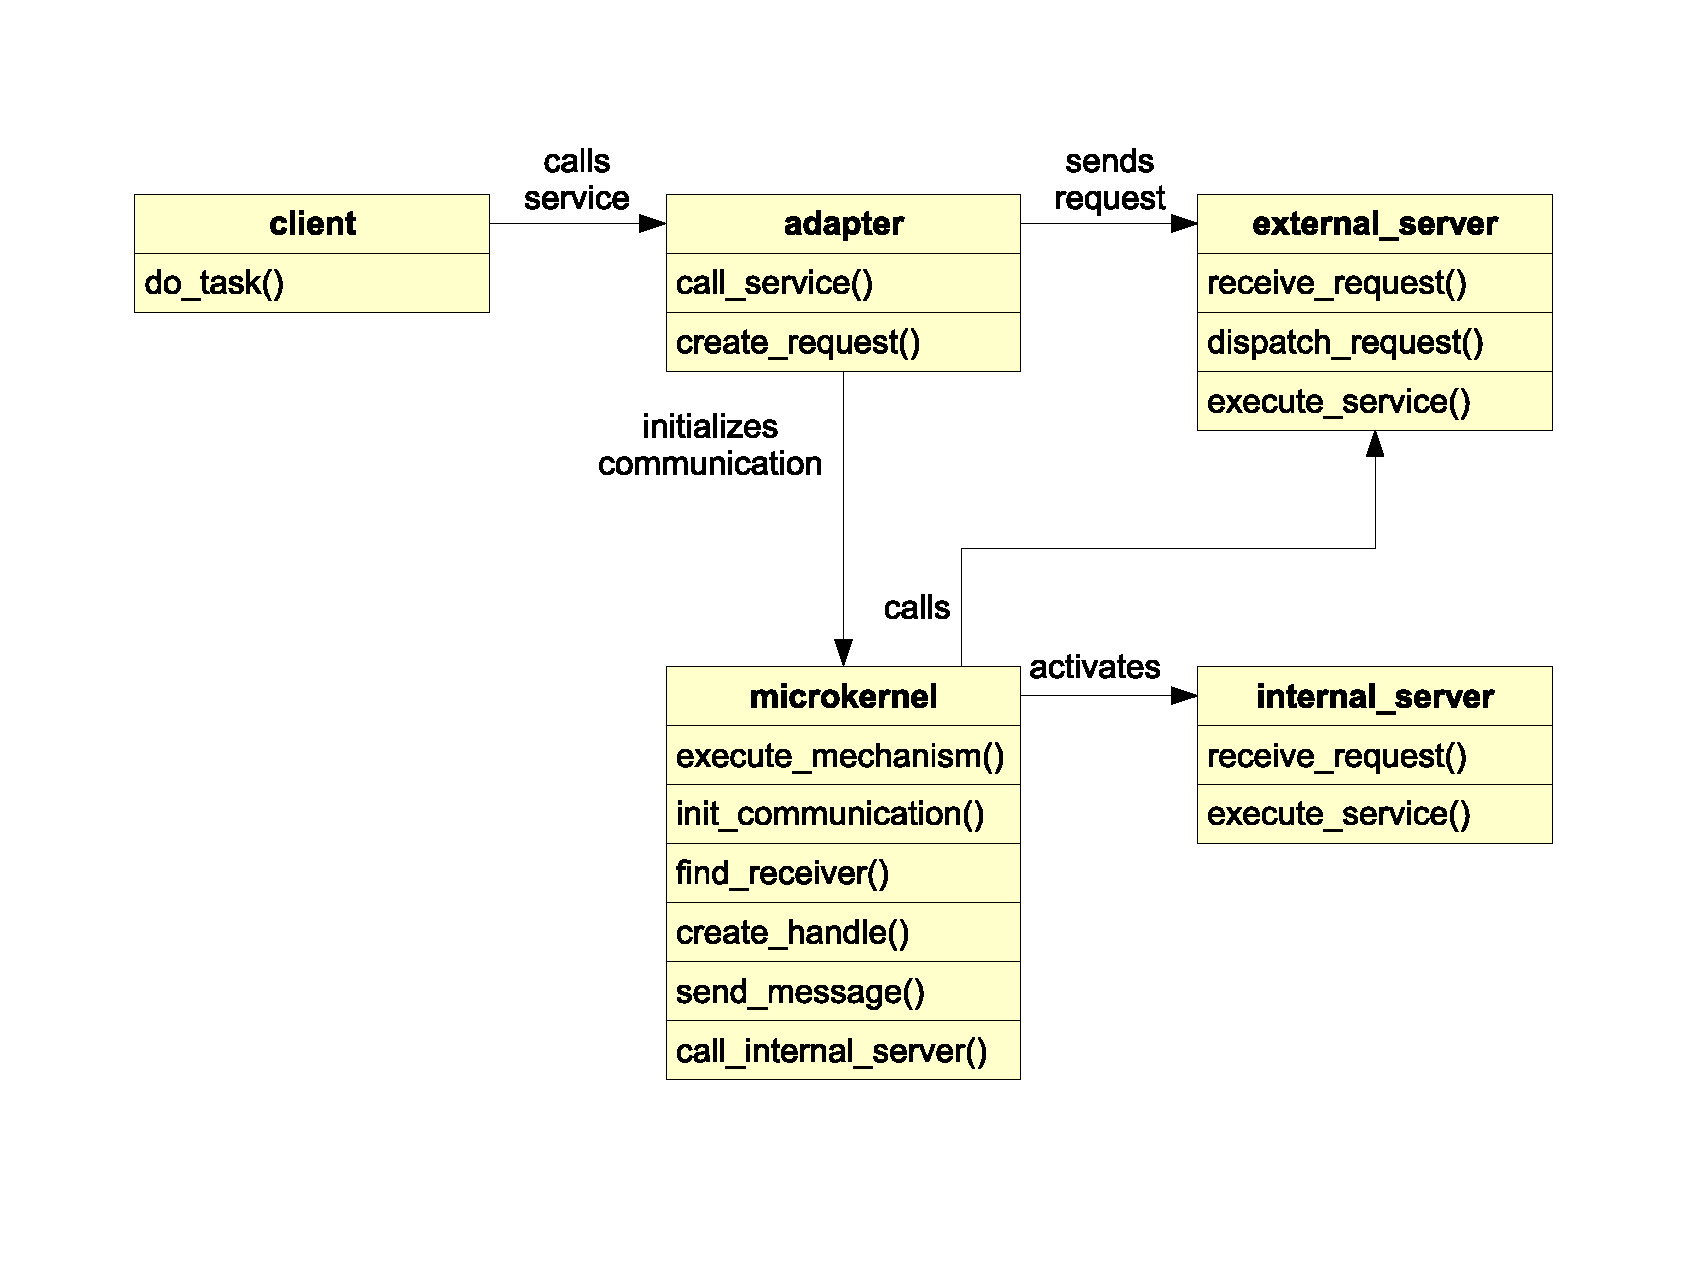
\includegraphics[scale=0.3]{vector/microkernel.eps}
        \caption{Microkernel Pattern}
        \label{microkernel_figure}
    \end{center}
\end{figure}

This pattern provides a \emph{Plug \& Play} environment and serves as base
architecture for many modern \emph{Operating Systems} (OS). Andrew S. Tanenbaum
recommends its use as well \cite{tanenbaum2001}.
